
  
\documentclass{exam}
\usepackage[utf8]{inputenc}
\usepackage{upgreek}
\usepackage[margin=1in]{geometry}
\usepackage{amsmath,amssymb}
\usepackage{multicol}
\usepackage{stmaryrd}
\usepackage{graphicx}
\usepackage{caption}
\usepackage{tikz}
\usepackage{dsfont}
\usepackage{enumitem}
\usepackage{hyperref}
\usepackage{float}
\usetikzlibrary{matrix}
\newcommand\tab[1][1cm]{\hspace*{#1}}
\pagestyle{head}
\firstpageheader{}{}{}
\runningheader{\examnum}{\class}{\name}
\runningheadrule
\newcommand{\class}{Fundamentos de bases de datos}
\newcommand{\term}{Facultad de Ciencias UNAM}
\newcommand{\examnum}{Practica 01 - Preguntas}
\newcommand{\examdate}{07/03/2022}
\newcommand{\name}{Jurassic Team}
\begin{document}

\noindent
\begin{tabular*}{\textwidth}{l @{\extracolsep{\fill}} r @{\extracolsep{6pt}} l}
\textbf{\class} & \textbf{\term}\\
\textbf{\examnum} & \textbf{\name}\\
\textbf{\examdate}
\end{tabular*}\\
\rule[2ex]{\textwidth}{2pt}

\section*{Preguntas}

\begin{questions}
	\question ¿Qué otros SMBD existen actualmente en el mercado?
	
	\question ¿Cuáles son las principales diferencias con PostgreSQL?
	
	\question ¿Por qué una empresa debería escoger una base de datos open source?
	
	\question ¿Cuáles son las ventajas, para un DBA el trabajar con un SMBD, open source?
	
	\question Describir a detalle qué es y para que sirve Docker y dar al menos 2 ejemplos de cómo podemos utilizar esta herramienta.
	
	\question ¿Qué son las bases de datos NoSQL? Menciona 3 ventajas y desventajas contra las bases relacionales.
\end{questions}

\noindent
\rule[2ex]{\textwidth}{2pt}

\section*{Respuestas}
\begin{questions}
	\question 
	\begin{itemize}
		\item Adaptative Server Anywhere
		\item Adaptative Server Enterprise
		\item ANTs Data Server
		\item DB2
		\item Firebird
		\item Informix
		\item HSQLDB
		\item Ingres
		\item InterBase
		\item SapDB
		\item MaxDB
		\item Microsoft SQL Server
		\item MySQL
		\item Oracle
		\item SmallSQL
		\item SQLite
		\item Microsoft Access
	\end{itemize}
	
	\question Postgre es un SMBD de código libre y completamente gratuito como no lo es, por ejemplo, Oracle
	Al ser un SMBD libre, este no cuenta con un soporte o asistencia oficial como si lo cuenta por ejemplo: Microsoft SQL Server, Microsoft Access, Oracle.
	Al estár diseñado específicamente para ambientes con alto volumen de datos, este puede parecer lente en relación a SMBD de pequeño y mediano tamaño
	Puede ser más complejo para el usuario ya que no presenta facilidad en comandos o sintaxis.
	
	
	\question El costo de una base de datos open source es muchas veces gratuito o bajo comparado con aquellas bases de datos privativas, lo que representa una gran ventaja para empresas de diversos tamaños, especialmente las startups.

A traves del tiempo se ha ido incorporando el soporte comercial en las bases de datos open source, por lo que es difícil encontrar un producto sin opciones de soporte.

Todos los proveedores de bases de datos deben de agregar características nuevas constantemente para seguir siendo competitivos. Algunas ventajas de las bases de datos open source son que innovan constantemente integrando nuevas características que diferencíen los productos de otros proveedores.

En general el software open source se crea bajo la colaboración de un grupo más grande de personas, lo que enriquece el desarrollo del mismo. Las bases de datos open source, además de esta colaboración, cuentan con el soporte brindado por algunos proveedores volviéndolas competitivas respecto a aquellas privativas y por ende atractivas para un gran número de empresas ya establecidas y emergentes.
	
	\question
	\begin{itemize}
	    \item Escalabilidad. El proyecto con el que trabaje el DBA puede comenzar siendo pequeño e instalar una configuración mínima para la base de datos. Dicha configuración puede irse ampliando en medida que la empresa lo requiera sin la necesidad de contratar un nuevo servicio con cada expansión.
	    
	    \item Modificación del Software. Al ser Open Source se puede ir modificando el código del SMBD para añadir o eliminar características. Para todo SMBD Open Source existe una comunidad de expertos que lo mantienen y si aparece alguna novedad en otro SMBD no faltará quien la importe. 
	    
	    \item Mayor alcance. Al ser libre es más fácil para las personas comenzar a estudiar ese sistema en particular, lo que aumenta la probabilidad de encontrar colaboradores que dominen el Software. 
	    
	    \item Compatibilidad. Por lo regular el software libre es compatible con una gran cantidad de dispositivos, lo que permite cambiar de equipos(ya sea locales o en la nube) sin necesidad de modificar en gran parte la configuración
	    
	\end{itemize}
	
	\question Docker es un Software que administra y ejecuta  contenedores. 
	
	Un contenedor es una pieza de Software que alberga una aplicación junto con los servicios que usa, logra esto virtualizando el sistema operativo. 
	
	Con Docker se puede correr Software sin cambiar nada en el sistema anfitrión, así se evitan instalaciones, conflictos de bibliotecas y se puede cambiar de versión con facilidad.
	
	Además que un contenedor preconfigurado garantiza que diferentes dispositivos estén ejecutando la misma versión con las mismas características.
	
	
	\begin{figure}[H]
	    \centering
	    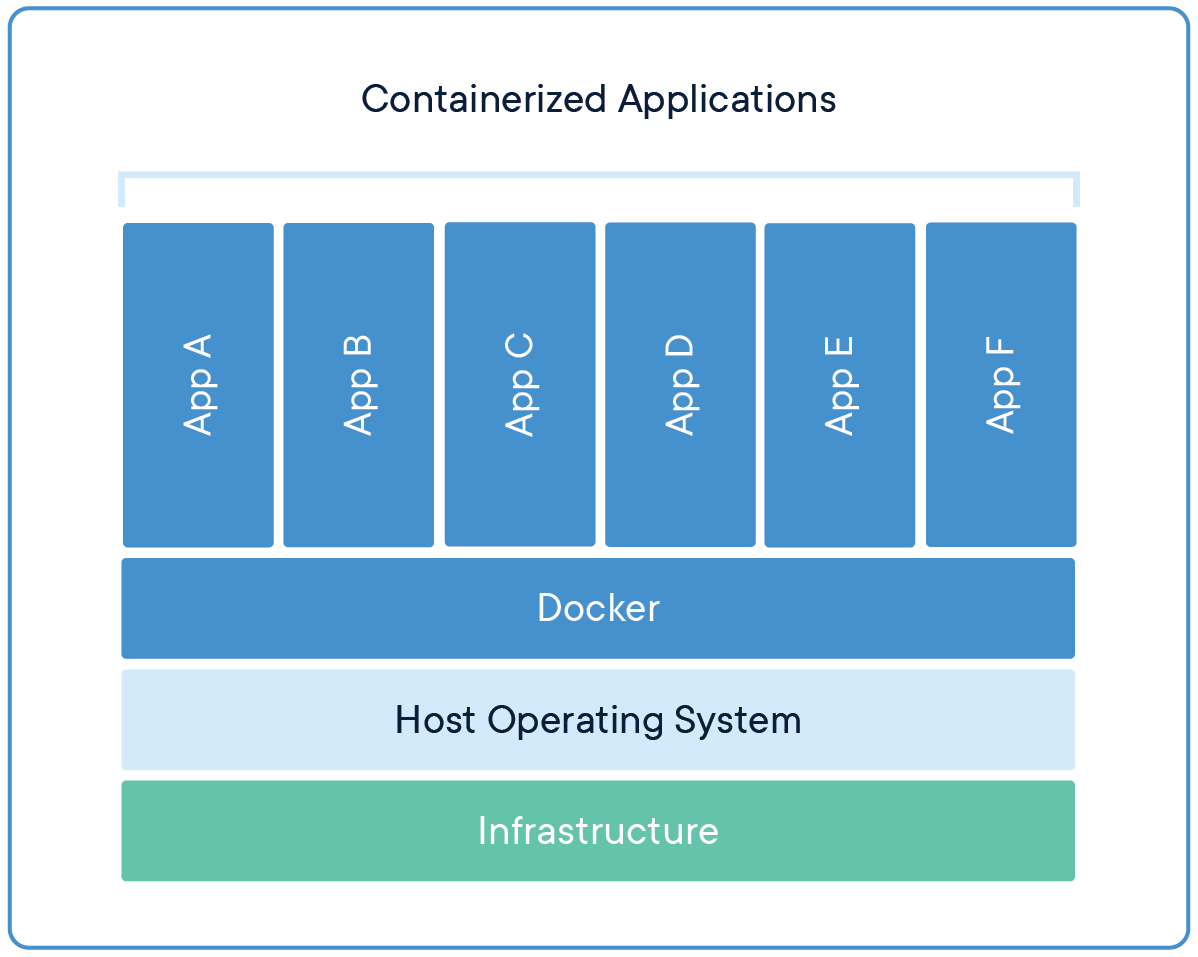
\includegraphics[width = 10cm]{imgCardenas/docker.png}
	\end{figure}
	
	Una forma muy común de usar Docker es para emular servidores en un ambiente aislado del sistema y así evitar conflictos al usar puertos. Por ejemplo Tomcat para aplicaciones, Wordpress o Django para web, PostgreSql, Oracle para bases de datos. 
	
	Otro uso bastante común es tener contenedores con diferentes versiones de lenguajes de programación. Por ejemplo tener java 8 y java 17 sin necesidad de configurar rutas y dependencias  específicas para cada compilador.
	
	
	\question Son sistemas de base de datos que almacenan información en esquemas con formato JSON. No tienen tablas, son llamadas colecciones y no necesariamente siguen el modelo Entidad-Relación.

\textbf{Ventajas}
\begin{enumerate}
	\item Al no tener una estructura definida el esquema se puede cambiar con facilidad sin perjudicar ningún registro.
	\item Su fácil escalabilidad y almacenamiento son superiores a SQL son la razon estos SMDB son usados para BigData.
	\item Al no tener estructura de tabla permite distintas maneras de visualizar los datos.
\end{enumerate}

\textbf{Desventajas}
\begin{enumerate}
	\item Consultas complejas pueden tardar mucho en ejecutarse, no soporta JOIN.
	\item No es posible garantizar la consistencia en los datos.
	\item No son suficientemente estables ni proporcionan atomicidad garantizada para ambientes de transacciones como sistemas bancarios.
\end{enumerate}
\end{questions}

\end{document}
